\documentclass[11pt]{article}
\usepackage[a4paper,margin=1in]{geometry}
\usepackage{amsmath,amssymb,amsthm}
\usepackage{booktabs}
\usepackage{graphicx}
\usepackage{hyperref}
\usepackage[numbers]{natbib}
\usepackage{array}
\usepackage{caption}

% Melhorar tipografia matemática
\hypersetup{colorlinks=true,linkcolor=blue,citecolor=blue,urlcolor=blue}
\setlength{\abovedisplayskip}{8pt}
\setlength{\belowdisplayskip}{8pt}
\setlength{\abovedisplayshortskip}{6pt}
\setlength{\belowdisplayshortskip}{6pt}

\title{Gauge Selection and Reachability\\in Rational Certificate Search}
\author{Jos\'e Cl\'audio da Silva Junior\\
\small State University of Londrina (UEL), Brazil\\
\small Electrical Engineering (B.Eng., 2016); Electronic Systems and Instrumentation (M.Sc., 2018)}
\date{May 2026}

\begin{document}
\maketitle

\begin{abstract}
We study how representation affects rational certificate search in creative telescoping.
Experiments across multiple hypergeometric families suggest that gauge selection can
change a search problem from unreachable to reachable under fixed ansatz budgets.
We further show that recurrence-derived denominator guidance substantially reduces
search cost once reachability is established.
\end{abstract}

\section{Introduction}
Creative telescoping reduces a hypergeometric summation identity to finding a rational function $R(n,k)$ satisfying
\[
F(n+1,k)-F(n,k)=\Delta_k\!\left[R(n,k)F(n,k)\right].
\]
Classical results establish algorithmic solvability for broad holonomic classes \cite{wilf1992,zeilberger1990,petkovsek1996,chyzak2000}. However, practical search is bounded by an ansatz: denominator candidates, maximum numerator degree, and recurrence order.

The central empirical observation is representation-dependent reachability:
\[
\text{same identity} \Rightarrow \text{different gauge} \Rightarrow \text{reachable vs. unreachable under the same budget.}
\]
Two phenomena are separated throughout:
\begin{itemize}
\item \textbf{Phenomenon A (reachability):} whether a certificate is found under a fixed budget.
\item \textbf{Phenomenon B (cost):} how expensive search is once a reachable gauge is used.
\item \textbf{Phenomenon C (transfer):} whether structural guidance generalizes across independent families.
\end{itemize}

\begin{figure}[htbp]
\centering
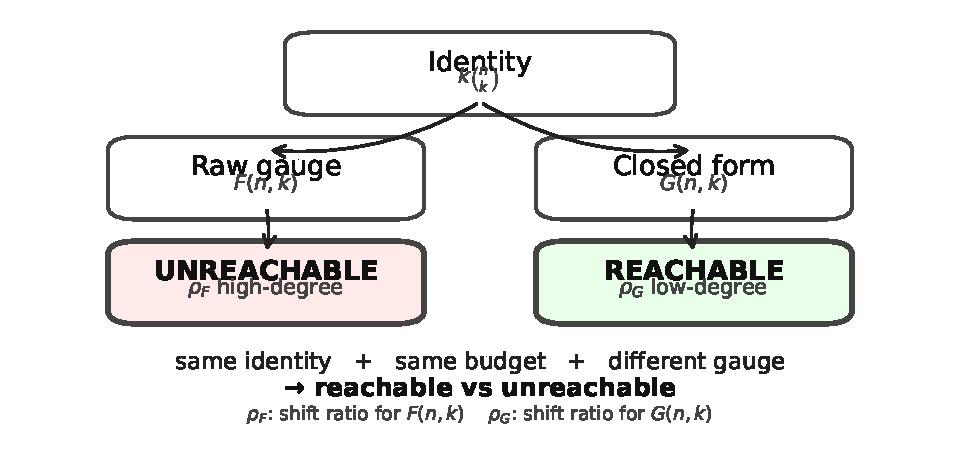
\includegraphics[width=\linewidth]{figure1.pdf}
\caption{The core observation: same identity and same budget, but different gauges lead to qualitatively different reachability outcomes.}
\label{fig:core-observation}
\end{figure}

\section{Related Work}
Creative telescoping and WZ methods are foundational in symbolic summation \cite{wilf1992,zeilberger1990,petkovsek1996}. Extensions to broader holonomic settings and algorithmic implementations are well-developed \cite{chyzak2000,kauers2011,schneider2007}. D-finite and holonomic function theory provides the structural framework for guaranteed recurrence existence \cite{stanley1980,lipshitz1989}. Standard references in symbolic computation and hypergeometric summation include \cite{geddes1992,koepf2014}.

Most prior work emphasizes existence, completeness classes, and algorithm design. Our contribution is orthogonal: under bounded ansatz regimes, representation choice (gauge) appears to govern practical reachability, and recurrence-derived denominator guidance appears to reduce cost substantially.

\section{Background and Definitions}
\subsection{Families}
We study:
\begin{itemize}
\item Binomial-power: $F_r(n,k)=\binom{n}{k}^r$, $r\in\{1,2,3,4\}$.
\item Weighted-binom: $F(n,k)=k\binom{n}{k}$ with closed-form normalized gauge $G(n,k)=\dfrac{k\binom{n}{k}}{n2^{n-1}}$.
\item Central Delannoy family (independent order-2 recurrence benchmark).
\end{itemize}

\subsection{Gauge}
Given hypergeometric $F(n,k)$, any $G(n,k)=c(n,k)F(n,k)$ with rational $c$ is
a gauge-transformed summand representation. We compare raw, closed-form, and
recurrence-LHS gauges.

\subsection{Reachability under budget}
Fix budget $B=(D,d,s)$ with denominator set $D$, max certificate degree $d$, and max recurrence order $s$. A certificate is reachable under $B$ iff search finds rational $R(n,k)$ within $B$ and symbolic telescoping verification succeeds.

\section{Structural Intuition}
Let $\rho_F(n,k)=F(n+1,k)/F(n,k)$. Telescoping coefficients inherit complexity from $\rho_F$. Under raw combinatorial gauges, high-degree factors often persist; under closed-form normalization,
\[
\rho_G=\frac{c(n+1,k)}{c(n,k)}\rho_F,
\]
which can cancel dominant factors and lower certificate complexity. This motivates gauge selection as symbolic preconditioning.

\section{Phenomenon A: Gauge Sensitivity and Reachability}
For $\sum_k k\binom{n}{k}=n2^{n-1}$ (guided denominator ansatz, max degree 4):

\begin{table}[htbp]
\centering
\small
\begin{tabular}{lccrr}
\toprule
Gauge & Reachable & Degree & {Equations solved} & {Median time (s)} \\
\midrule
raw & NO & --- & 533 & 1.530 \\
closed\_form & YES & 1 & 10 & 0.033 \\
recurrence\_lhs & NO & --- & 517 & 1.920 \\
\bottomrule
\end{tabular}
\caption{Gauge sensitivity under fixed budget for the weighted-binom identity.}
\label{tab:phenomenon-a}
\end{table}

Recovered closed-form certificate:
\[
R(n,k)=\frac{k-1}{2(k-n-1)}.
\]

This controlled intervention (one representation change, one outcome change) is consistent with a causal interpretation of gauge-dependent reachability.

\section{Phenomenon B: Guided Denominator Search Cost}
For $\sum_k \binom{n}{k}^r$ with closed-form gauge:

\begin{table}[htbp]
\centering
\footnotesize
\setlength{\tabcolsep}{3pt}
\begin{tabular}{rrrrrrrcc}
\toprule
{$r$} & {\shortstack{Baseline\\cands}} & {\shortstack{Guided\\cands}} & {\shortstack{Reduction\\(\%)}} & {\shortstack{Baseline\\time (s)}} & {\shortstack{Guided\\time (s)}} & {\shortstack{Time red.\\(\%)}} & {\shortstack{Reach-\\able?}} & {Verified} \\
\midrule
1 & 23 & 6 & 74 & 0.063 & 0.028 & 56 & YES & YES \\
2 & 27 & 6 & 78 & 8.890 & 1.610 & 82 & YES & YES \\
3 & 46 & 8 & 83 & 185.200 & 33.000 & 82 & NO & NO \\
4 & 51 & 9 & 82 & 421.200 & 77.400 & 82 & NO & NO \\
\bottomrule
\end{tabular}
\caption{Guided denominator selection reduces candidate set size and runtime in the binomial-power family.}
\label{tab:phenomenon-b}
\end{table}

Delannoy cross-family replication: baseline 22.617 s, guided 2.339 s (89.7\% reduction).

\section{Discussion}
\subsection{Qualitative boundary, not only speed}
Under bounded search, representation changes can move an instance across a qualitative reachability boundary, not merely accelerate an otherwise-successful run.

\subsection{Preconditioning analogy}
As numerical preconditioners improve linear-system geometry, gauge changes appear to improve symbolic search geometry by reducing certificate degree and denominator complexity.

\subsection{Link between A, B, and C}
Phenomenon A concerns feasibility under budget; Phenomenon B concerns efficiency within feasible regimes; Phenomenon C indicates transfer of structural guidance across families.

\section{Limitations and Open Questions}
\begin{itemize}
\item Guided denominator prediction is heuristic; no completeness proof is claimed.
\item Higher-order cases ($r=3,4$) remain unverified under current budgets.
\item Failure under budget $B$ is not non-existence.
\item Closed-form gauge selection is currently manual.
\item Experiments use univariate recurrences in $n$ (orders 1 and 2 in the present benchmarks); multivariate settings are open.
\end{itemize}

\section{Conclusion}
Representation strongly influences certificate reachability in the tested regime.
Once representation enables reachability, structural guidance promotes efficiency.
This yields a practical workflow for bounded symbolic search: first optimize
representation, then optimize denominator search.

\appendix
\section{Reproducibility}
Experiments are generated by \texttt{src/wz\_lab.py}, with JSON/CSV traces in \texttt{results/}. Negative results are retained with full metadata (gauge, denominator candidates, equations solved, runtime), enabling explicit reachability-boundary analysis.

Code, traces, and experiment scripts are available at:
\url{https://github.com/JoseClaudioSJr/gauge-reachability-symbolic-search}

\bibliographystyle{plainnat}
\bibliography{references}

\end{document}
